\vspace{-0.3cm}
\subsection*{B+ Tree - Overview}
\vspace{-0.1cm}

\noindent
A type of self-balancing tree data structure that maintains sorted data and allows for searches,
sequential access, insertions, and deletions in logarithmic time.
The B+ tree represents an index structure that is highly optimized for systems that read and write large blocks of data.

\noindent
\textbf{Root Level}
\begin{itemize}[noitemsep,leftmargin=*]
\item{The root node contains keys that act as separation values which divide its subtrees.}
\item{For instance, the key `39` separates the range of keys that are less than `39` and those that are greater than or equal to `39` but less than `788`.}
\end{itemize}

\noindent
\textbf{Intermediate Level}
\begin{itemize}[noitemsep,leftmargin=*]
\item{These nodes (also known as internal nodes) contain keys that similarly divide the range of keys.}
\item{Each key in the intermediate nodes corresponds to a pointer to a node in the level below.}
\end{itemize}

\noindent
\textbf{Leaf Level}
\begin{itemize}[noitemsep,leftmargin=*]
\item{The leaf nodes contain the actual records or pointers to the records. In your diagram, the leaf nodes contain a set of keys (ID) and their corresponding values (NAME).}
\item{Leaf nodes are linked to each other in a linked-list fashion, which makes range queries efficient as you can traverse these nodes sequentially.}
\end{itemize}



\noindent
\textbf{Characteristics of the B+ Tree in the Diagram}

\begin{enumerate}[noitemsep,leftmargin=*]
\item{All keys are stored in the leaf nodes}
\item{The leaf nodes of the tree form a linked list - easy to move between leafs. This is useful for full table scans, range searches, or sequential access.}
\item{The intermediate nodes guide the search. They contain keys and pointers that direct the search to the correct leaf node.}
\item{The tree is balanced - all leaf nodes are at the same level, ensures that all search operations require the same number of disk accesses.}
\item{The internal nodes only contain keys and not the full records, they can hold more keys and thus reduce the height of the tree.}
\end{enumerate}


\begin{center}
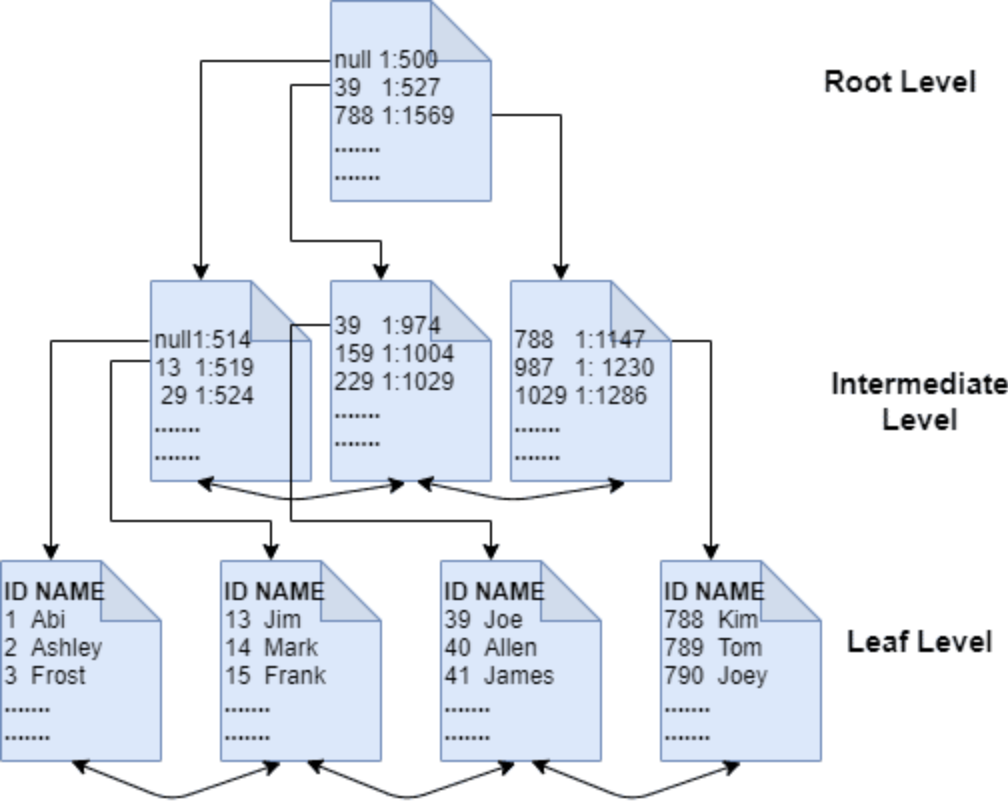
\includegraphics[width=8cm,height=4cm]{memory_related/b_tree/b_tree_img}
\end{center}

